\subsubsection{Set 4 - Lindemans Aalst}
\label{sec:PL3_Aalst4}
%TODO: tekst aanpassen
De opslag- en recetpiestatistieken zijn weergegeven in figuur \ref{fig:PL3ServeReceiveAalst4}. 

Bij de opslag komt het teken \# overeen met 0, + en / met 1, ! met 2, - en = met 3.

De foutieve opslagen, bij manuele invoer een = en bij AI-invoer een Serve Error (SE), zijn correct weergegeven.  Ook de perfecte opslag is hetzelfde. Bij de andere opslagen valt op dat de AI meer score 2 geeft en de manuele meer score 1.

De beoordeling van de receptie is op een andere wijze gedaan dan bij de manuele invoer. Bij de manuele invoer wordt er gebruik gemaakt van tekens, terwijl bij de AI-invoer gebruik wordt gemaakt van cijfers. Bij de receptie komt het teken \# overeen met 3, + en / met 2, ! met 1, - en = met 0.

De AI heeft bij geen enkele receptie een score van 0 gegeven. Bij de manuele invoer is dit wel het geval voor vijf recepties. Ook bij de andere scores wordt duidelijk dat de manuele invoer kritischer is dan de AI.

\begin{figure}[ht]
\centering
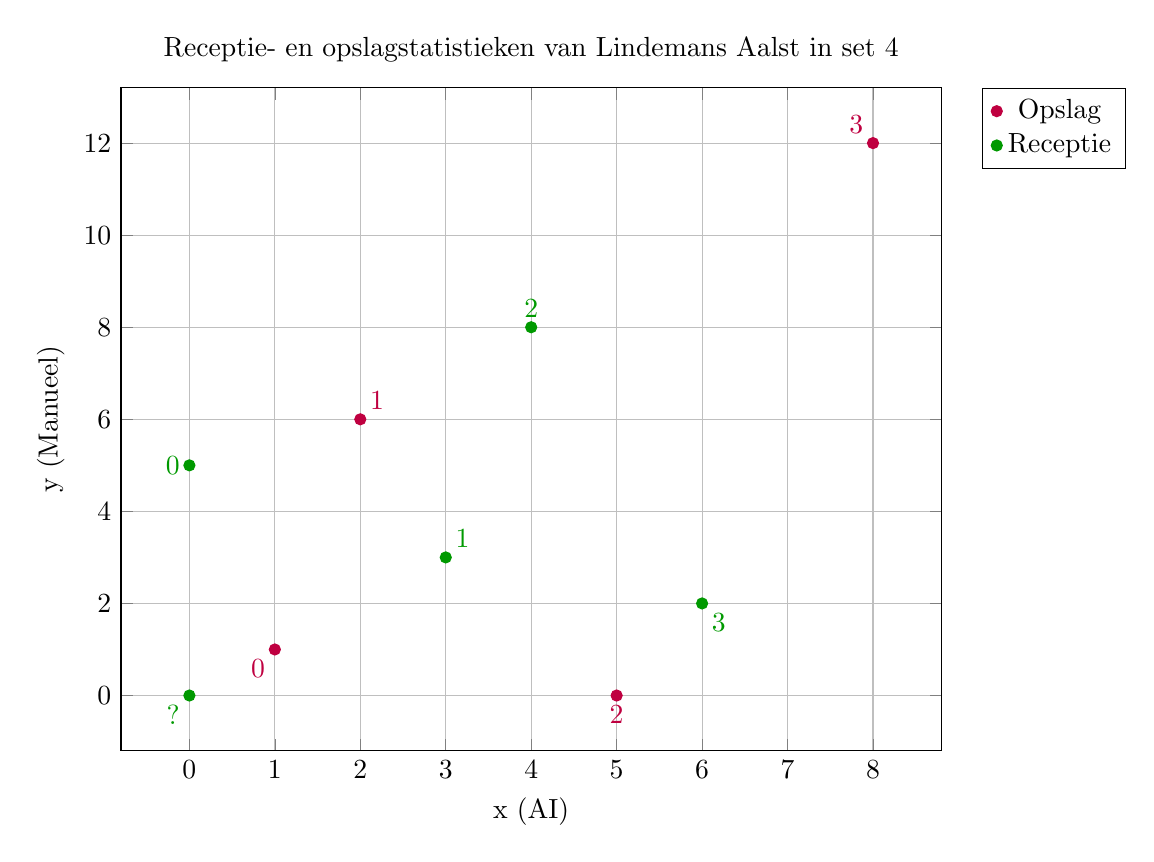
\begin{tikzpicture}
  \begin{axis}[
    title={Receptie- en opslagstatistieken van Lindemans Aalst in set 4},
    xlabel={x (AI)},
    ylabel={y (Manueel)},
    grid=major,
    legend style={at={(1.05,1)}, anchor=north west},
    width=12cm,
    height=10cm,
    enlargelimits=0.1,
  ]

  % Opslag
  \addplot[
    only marks,
    mark=*,
    color=purple,
  ] table {
    x y
    1 1
    2 6
    5 0
    8 12
  };
  \addlegendentry{Opslag}

  % Labels opslag
  \node at (axis cs:1,1) [anchor=north east, purple] {0};
  \node at (axis cs:2,6) [anchor=south west, purple] {1};
  \node at (axis cs:5,0) [anchor=north, purple] {2};
  \node at (axis cs:8,12) [anchor=south east, purple] {3};

  % Receptie
  \addplot[
    only marks,
    mark=*,
    color=green!60!black,
  ] table {
    x y
    6 2
    4 8
    3 3
    0 5
    0 0
  };
  \addlegendentry{Receptie}

  % Labels receptie
  \node at (axis cs:6,2) [anchor=north west, green!60!black] {3};
  \node at (axis cs:4,8) [anchor=south, green!60!black] {2};
  \node at (axis cs:3,3) [anchor=south west, green!60!black] {1};
  \node at (axis cs:0,5) [anchor=east, green!60!black] {0};
  \node at (axis cs:0,0) [anchor=north east, green!60!black] {?};

  \end{axis}
\end{tikzpicture}
\caption{AI invoer versus manuele invoer, ingedeeld in opslag en receptie, voor Lindemans Aalst in set 4.}
\label{fig:PL3ServeReceiveAalst4}
\end{figure}

In tabel \ref{tab:PL3SetAalstMan4} en \ref{tab:PL3DigAalstMan4} zijn de manueel ingevoerde spelverdelings- en verdedigingsstatistieken weergegeven. De statistieken van de AI zijn weergegeven in tabel \ref{tab:PL3SetDigAalstAI4}.
Bij de spelverdelingsstatistieken valt op dat Max Schulz een actie meer heeft bij de AI-invoer dan bij de manuele invoer. Bij het bekijken van de video valt dan wel op dat hij effectief een actie meer heeft uitgevoerd. 

Bij de verdedigingsstatistieken zijn er verschillende hoeveelheden. Bij 2 van de spelers is het wel correct. Bij de andere is er een verschil van 2 tot 1 actie minder door de AI-invoer.

\begin{table}[ht!]
    \centering
    \scriptsize
    \begin{tabular}{|l|c|c|c|c|c|c|c|c|}
        \hline
        \textbf{Speler} & *E\% & Tot & = & / & - & ! & + & \# \\ \hline
        Bert Dufraing & 100\% & 1 &  &  &  & & 1 &  \\ 
        Max Schulz & 100\% & 1 &  &  &  & & & 1 \\ 
        Lucas Lorente Lòpez & 100\% & 16 &  &  &  &  & 15 & 1 \\ 
        Matis Verwimp &100\% & 1 & & & & & 1 & \\\hline
    \end{tabular}
    \caption[Manueel ingevoerde spelverdelingsstatistieken voor Lindemans Aalst in set 4]{\label{tab:PL3SetAalstMan4}Manueel ingevoerde spelverdelingsstatistieken voor Lindemans Aalst in set 4.}
\end{table}

\begin{table}[ht!]
    \centering
    \scriptsize
    \begin{tabular}{|l|c|c|c|c|c|c|c|c|}
        \hline
        \textbf{Speler} & *E\% & Tot & = & / & - & ! & + & \# \\ \hline
        Bert Dufraing & 50\% & 2 &  & 1 & 1 &  &  & \\ 
        Berre Peters & 50\% & 4 & 1 & 1 & 1 & & 1 &  \\ 
        Max Schulz & 0\% & 1 & 1 &  &  &  &  & \\ 
        Nezar Harouk & 0\% & 1 &  &  & 1 &  &  &  \\ 
        Lucas Lorente Lòpez & 0\% & 1 &  &  & 1 &  &  & \\ \hline
    \end{tabular}
    \caption[Manueel ingevoerde verdedigingsstatistieken voor Lindemans Aalst in set 4]{\label{tab:PL3DigAalstMan4}Manueel ingevoerde verdedigingsstatistieken voor Lindemans Aalst in set 4.}
\end{table}

\begin{table}[ht!]
  \centering
  \scriptsize
  \begin{tabular}{|l|c|c|c|c|c|c|c|} \hline
    \textbf{Speler} & Ast & TA & SE & PCT & DS &  DE \\ \hline
    Bert Dufraing &  & 1 &  & 0\% & 1 &  \\
    Berre Peters &   &   &   &   & 2 &   \\
    Max Schulz &  & 2 &  & 0\% &   &   \\
    Nezar Harouk &   &   &   &   &  1 &   \\
    Lucas Lorente Lòpez & 10 & 16 &  & 62\% & 1 &  \\
    Matis Verwimp &  & 1 & & 0\% &   &   \\ \hline
  \end{tabular}
 \caption[Spelverdelings- en verdedigingsstatistieken gemaakt door Balltime AI voor Lindemans Aalst in set 4]{\label{tab:PL3SetDigAalstAI4}Spelverdelings- en verdedigingsstatistieken gemaakt door Balltime AI voor Lindemans Aalst in set 4.}
\end{table}

De aanvalsstatistieken in deze set worden weergegeven in de tabellen \ref{tab:PL3AttAalstMan4} en \ref{tab:PL3AttBlockAalstAI4}. De blokstatistieken zijn weergegeven in de tabellen \ref{tab:PL3BlockAalstMan4} en \ref{tab:PL3AttBlockAalstAI4}. De AI-invoer geeft aan dat Lucas Lorente Lòpez ook één keer aanvalt, terwijl de manuele invoer dit niet aangeeft. Bij het bekijken van de video is duidelijk dat hij dit effectief niet doet. De hoeveelheid correcte aanvallen is bij beide hetzelfde aantal.

Bij de blokstatistieken is er een zeer groot verschil aanwezig. De AI geeft aan dat er maar één blok doorheen de hele set is, terwijl de manuele invoer er negen in totaal aangeeft.

De kwaliteit van aanvallen en blokkeringen worden niet beoordeeld door de AI. 

\begin{table}[ht!]
    \centering
    \scriptsize
    \begin{tabular}{|l|c|c|c|c|c|c|c|c|}
        \hline
        \textbf{Speler} & *E\% & Tot & = & / & - & ! & + & \# \\ \hline
        Berre Peters & 43\% & 7 & 1 &  &  & & 2 & 4 \\ 
        Max Schulz & 20\% & 5 & 1 &  & 1 & 1 & & 2 \\ 
        Mihkel Varblane & -100\% & 1 &  & 1 &  &  &  & \\ 
        Alvaro Gimeno Rubio & 43\% & 7 &  & 1 & & & 2 & 4 \\ \hline
    \end{tabular}
    \caption[Manueel ingevoerde aanvalsstatistieken voor Lindemans Aalst in set 4]{\label{tab:PL3AttAalstMan4}Manueel ingevoerde aanvalsstatistieken voor Lindemans Aalst in set 4.}
\end{table}

\begin{table}[ht!]
    \centering
    \scriptsize
    \begin{tabular}{|l|c|c|c|c|c|c|c|c|}
        \hline
        \textbf{Speler} & *E\% & Tot & = & / & - & ! & + & \# \\ \hline
        Max Schulz & -100\% & 1 & 1 &  &  &  &  & \\
        Nezar Harouk & -75\% & 4 & 3 & &  & 1 &  & \\ 
        Mihkel Varblane & -33\% & 3 & 2 &  &  & &  & 1 \\ 
        Alvaro Gimeno Rubio & -100\% & 1 & 1 &  &  &  &  & \\  \hline
    \end{tabular}
    \caption[Manueel ingevoerde blokstatistieken voor Lindemans Aalst in set 4]{\label{tab:PL3BlockAalstMan4}Manueel ingevoerde blokstatistieken voor Lindemans Aalst in set 4.}
\end{table}

\begin{table}[ht!]
  \centering
  \scriptsize
  \begin{tabular}{|l|c|c|c|c|c|c|c|c|c|c|c|} \hline
    \textbf{Speler} &  K & E & TA & Atk\% & Kill\% & Error\% & BS & BA & BE \\ \hline
    Berre Peters & 4 & 1 & 7 & 0.43 & 57\% & 14\% &  &  & \\
    Max Schulz & 2 & 1 & 5 & 0.20 & 40\% & 20\% &  &  & \\
    Mihkel Varblane &  & 1 & 1 & -1.00 & 0\% & 100\% & 1 & & \\
    Alvaro Gimeno Rubio & 4 & 1 & 7 & 0.43 & 57\% & 14\% &  &  & \\
    Lucas Lorente Lòpez &  &  & 1 & 0 & 0\% & 0\% &  &  &\\ \hline
  \end{tabular}
  \caption[Aanvals- en blokstatistieken gemaakt door Balltime AI voor Lindemans Aalst in set 4]{\label{tab:PL3AttBlockAalstAI4}Aanvals- en blokstatistieken gemaakt door Balltime AI voor Lindemans Aalst in set 4.}
\end{table}
